\documentclass{article}
\usepackage[utf8]{inputenc}


\usepackage[margin=1in,top=1in,bottom=1in]{geometry}
\usepackage[pdftex]{graphicx}
\usepackage{tikz}
\usetikzlibrary{shapes,arrows,patterns,decorations.pathreplacing, decorations.markings,positioning,calc,decorations.pathmorphing}
\usepackage{setspace}
\usepackage{epstopdf}
\usepackage{caption}
\usepackage{enumitem}
\usepackage{pdfpages}
\usepackage{placeins}
\usepackage{subcaption}
\usepackage{amsmath}
\usepackage{empheq}
\usepackage{cancel}
\usepackage{xcolor}
\usepackage{etoolbox}
\usepackage{soul}
\usepackage{listings}
\lstset{
       basicstyle=\footnotesize\ttfamily,
       backgroundcolor=\color{lightGray},
       frame=single,
%        basicstyle=\footnotesize\sf,
       captionpos=b,
       tabsize=2,
       keepspaces=true,
       breaklines=true,
       postbreak=\mbox{\textcolor{red}{$\hookrightarrow$}\space},
  }
\usepackage{color}
\definecolor{lightGray}{rgb}{0.95,0.95,0.95}

% The call to include hyperref must be after most of the other packages are called.
% One notable exception it that hyperref must come before cleveref.
% Basically keep these two packages at the end of the \usepackage{} calls, in this order.
\usepackage[pdftex,
            hidelinks,
            pdfauthor={Evan Brunton},
            pdftitle={MAE 3302 --- Project Part 1},
            pdfsubject={Thermodynamics 2}
            ]{hyperref}


\usepackage[capitalize]{cleveref}
\newcommand{\creflastconjunction}{,~and~} % page 12 of the manual to get serial comma correct

\graphicspath{{Figures/}}

\title{Conceptual Design of a Combined Gas Turbine and Steam Turbine Power Plant}

\date{\today}

\author{Evan B, Brunton\\[2ex]
    UCCS Department of Mechanical\\
    and Aerospace Engineering
}

\begin{document}

\maketitle

\pagebreak

\section{Introduction}

    This study will analyze a conceptually combined gas and steam turbine power plant and seek to maximize efficiency. The gas and steam turbine mechanisms will be modeled using ideal Brayton and Rankine thermodynamic cycles with component efficiency factored into the processes. The Brayton cycle models the gas turbine part of the power plant. In the Brayton cycle atmospheric air is first pumped into a combustion chamber raising the pressure of the gas. Combustion is then modeled as heat entering the system in an isobaric process, the temperature rises, but the pressure is constant. The now pressurized and heated gas is put through a turbine to generate work. However, the gas is still extremely hot and more work can be extracted from that energy. The hot gas is then put through a heat exchanger which inputs heat into the Rankine cycle. The Rankine cycle models a steam turbine, which uses the spent heat from the Brayton cycle to heat water into steam that drives a turbine providing more work out. Figure 1 diagrams the inputs/outputs and flow of the two cycles.
    
\begin{figure}[!htbp]
\centering
  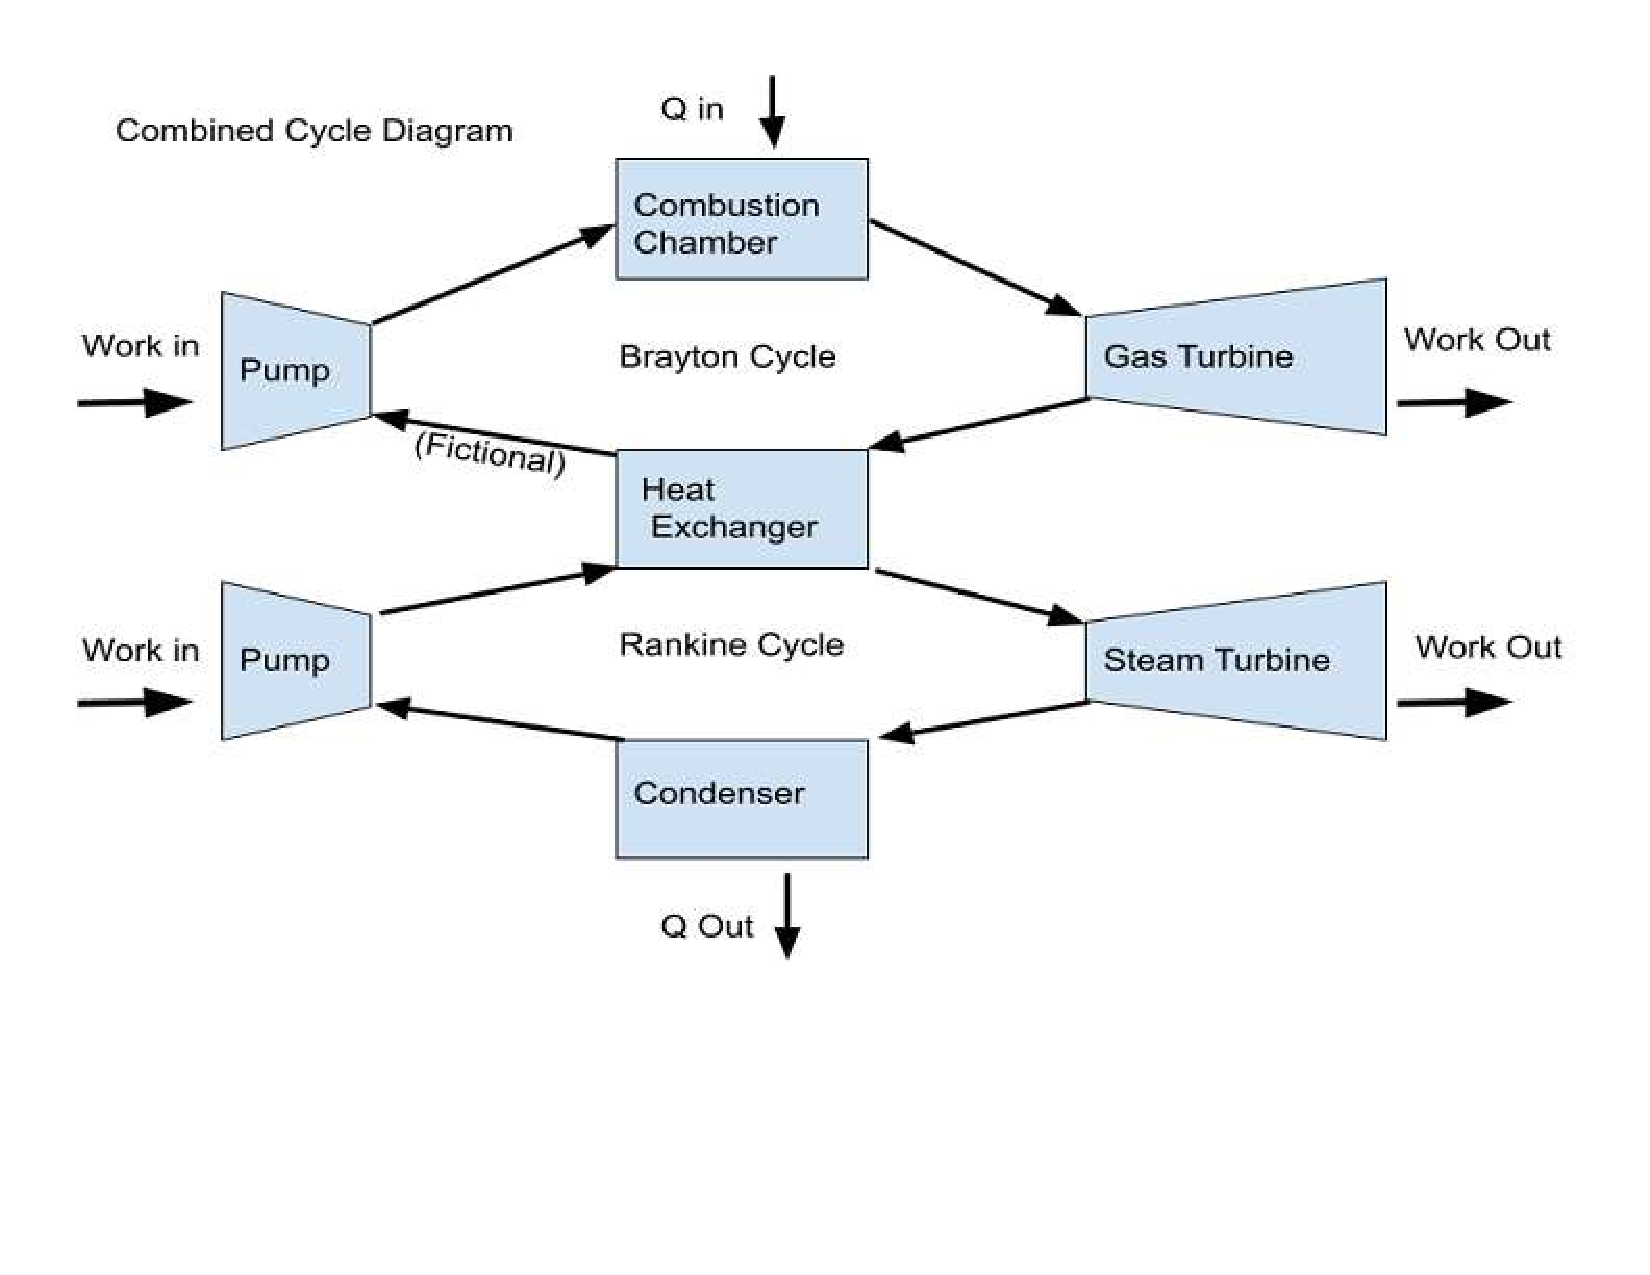
\includegraphics[page=1,trim=10mm 40mm 10mm 0mm,clip,width=0.99\textwidth]{Combined Cycle Diagram (1).pdf}
  \caption{}
  \label{fig:epsfig}
\end{figure}

\FloatBarrier

The requested design parameters of the power plant and the efficiency of the components are as follows:

\begin{figure}[htbp]
  \centering
  \begin{subfigure}[t]{0.45\textwidth}
    \centering
  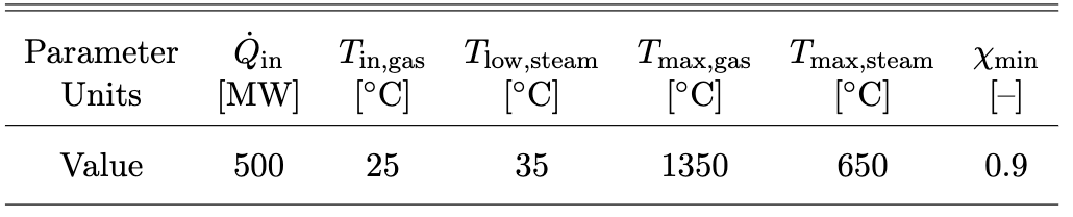
\includegraphics[page=1,trim=0mm 0mm 0mm 0mm,clip,width=0.99\textwidth]{Figures/png2pdf (1).pdf}
  \caption{Component efficencies}
  \label{fig:epsfig}
\end{subfigure}%
  \begin{subfigure}[t]{0.45\textwidth}
  \centering
  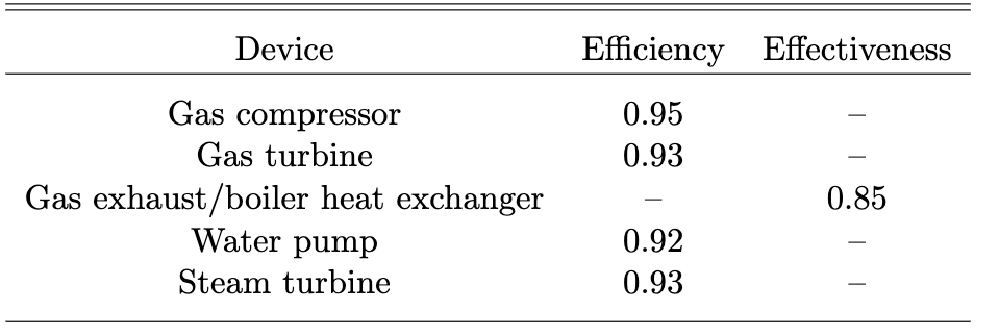
\includegraphics[page=1,trim=0mm 0mm 0mm 0mm,clip,width=0.99\textwidth]{Figures/png2pdf.pdf}
  \caption{These are the overall design requirements}
  \label{fig:pdffig}
  \end{subfigure}%
  \caption{}
  \label{fig:testfig}
\end{figure}

\FloatBarrier
In order to increase the efficiency of the entire powerplant both cycles should have their output maximised. The Brayton cycle's efficiency ultimately depends on the pressure ratio. However, as the temperature and pressure increase the costs and feasibility of building a compressor that can handle the high pressure and temperatures rises exponentially the efficiency gain levels off, compressing gas concentrates the heat energy, and compressing at a high temperature takes significantly more energy than a low-temperature gas. Eventually, the work required to compress the atmospheric air overcomes the work generated by the turbine.
A second compressor and inter-cooler can be installed to reduce the work required to compress the gas and the temperature limits of the compressor. Before compressing the gas to its final pressure, the gas is run through a heat exchanger in a constant pressure process. The excess heat can be used in other processes, and not as much work will be required to get the gas to the required pressure.
The Rankine cycle also has to deal with realistic pressure and temperatures requirement determined by our current material science. So increasing temperature and pressure to overcome other losses is not a realistic way to maximize efficiency. The cycle also has to deal with using a two-phase liquid gas mixture throughout the process. A pump can only deal with non-saturated water, and the turbine can only deal with steam at a higher than 90\% quality. So to maximize efficiency one would have to edge their way around the vapor dome, keeping the temperature from getting too high, keeping the compressor from having to over-compress the liquid, and the turbine quality above 90\%.
In order to edge along the vapor dome for the Rankine cycle a reheat cycle and a second turbine can be added. This way temperature doesn't have to get too high and a lower initial temperature can be used. The higher the difference in low and high temperatures will increase the amount of work that can be extracted from the steam. Excess heat energy from other parts of the powerplant, like the combustion chamber, that would have been lost to the atmosphere can be used in this reheat step. This would increase the work generation per unit of energy. This energy comes from burning expensive and polluting gas. 
This report will determine the increase in efficiency from using these extra components. From the results, the efficacy of installing them can be extrapolated from projected fuel savings against the projected cost.

\begin{figure}[!htbp]
\centering
  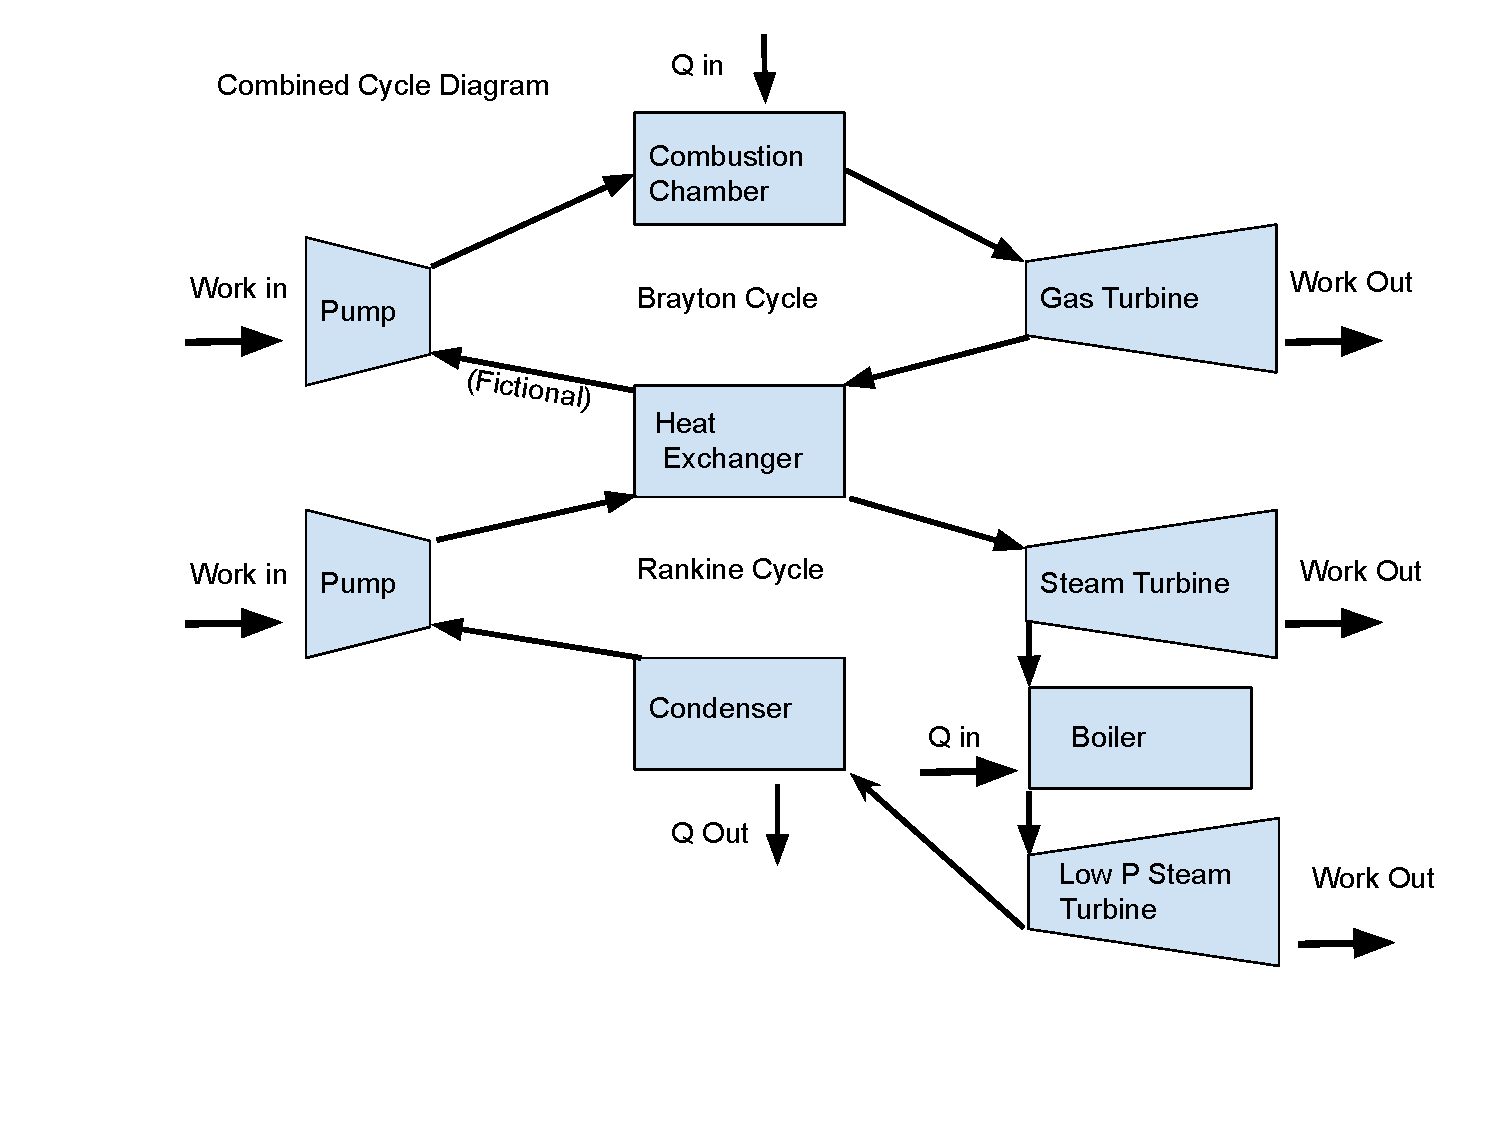
\includegraphics[page=1,trim=10mm 0mm 10mm 0mm,clip,width=0.99\textwidth]{Figures/Copy of Combined Cycle Diagram.pdf}
  \caption{}
  \label{fig:epsfig}
\end{figure}

\FloatBarrier

\section{Modeling Brayton}

The attached Python script uses CoolProp, a database with experimental values for water and air at incremental states. Using the design requirements of the power plant for all the states of the working fluid/gas can be found. After factoring in the efficiency of the components the enthalpy of the materials can be used to find the work out, work in, and Q-in can be used to find the thermal efficiency of the two cycles. The Brayton cycle model with the following initial conditions; a compressor efficiency of 0.95 and a turbine efficiency of 0.93 will have a thermal efficiency of 32.98 \%.
\begin{itemize}
\item  low pressure = 101325 pa
\item Minimum temp of gas = 25 Celsius
\item compressor ratio = 6
\item Maximum temp of gas = 1350 Celsius
\end{itemize}

However, if an intercooler and second compressor are added to the cycle, with the initial compressor having a pressure ratio of 3, and the intercooler cooling the gas to 25 Celsius (25 Celsius was used for simplicity, an inter cooler would only quickly cool a gas to a temperature above the environmental temperature) the system will have a thermal efficiency of 35.67 \%.  A 2.69 percent increase may not sound like a lot of savings, but most of the cost of running a power plant is fuel, and a 2.69 \% reduction in fuel costs is a serious amount of money. The Following T-S diagram shows the cycle.

\begin{figure}
    \centering
    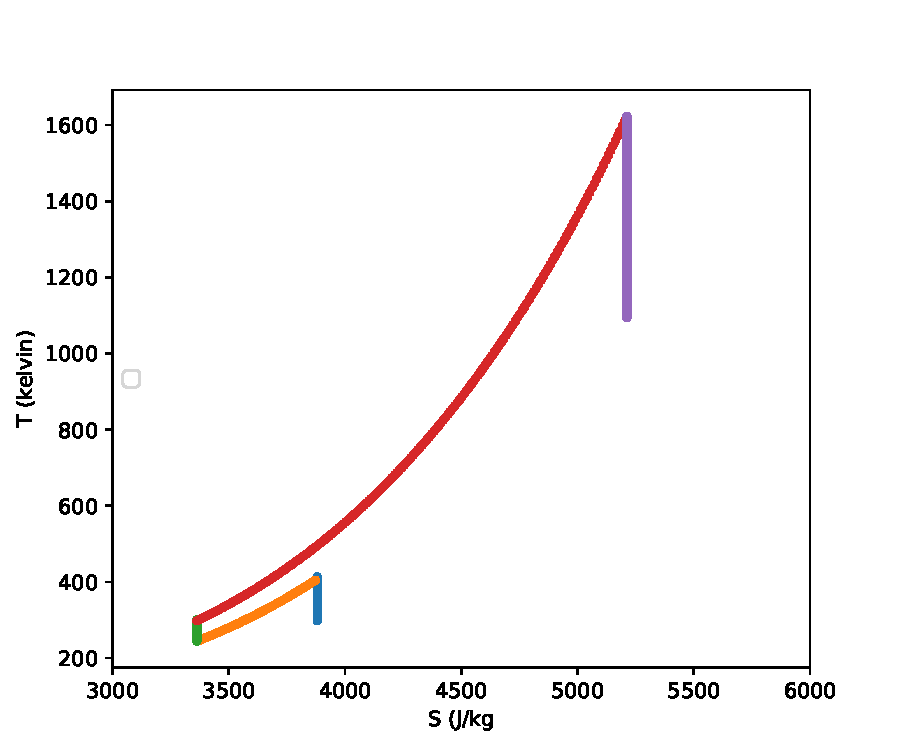
\includegraphics{BraytonDiagramInitial.pdf}
    \caption{}
    
    \label{fig:my_label}
\end{figure}

\FloatBarrier

\section{Modeling Rankine}
The material properties at all states of the Rankine cycle can be found using CoolProp. Then using the enthalpy of the water at the various states work done by the pump, and work out of the turbines can be compared with Q-in.(will update values in submission 3 to project values) Using the following state conditions a pump efficiency of 0.92 and a turbine efficiency of 0.93 the thermal efficiency of the cycle is 40.69 \% is found.
\begin{itemize}
\item  low pressure = 6000 pa
\item high pressure = 10000000 pa
\item low temperature = 35 Celsius
\item high temperature = 650 Celsius
\end{itemize}

However, the minimum quality of the water exiting the turbine is specified to be larger than 90 \%, so as not to break it. Without a reheat and a second turbine, the quality at the turbine exit is 83.5 \%. If the water leaves the first turbine at 700000 pa and is reheated to the maximum temperature and then sent through a second turbine until it reaches the low pressure the thermal efficiency is 46.93 \%. Not only does the reheating step maintain the quality of the material, so the turbines aren't damaged, but it increases the thermal efficiency by a whole 6.24 \%. Figure 4 shows the modified Temperature and entropy graph of the cycle, the two big drop-offs are the isentropic expansions in the turbines.

\begin{figure}
    \centering
    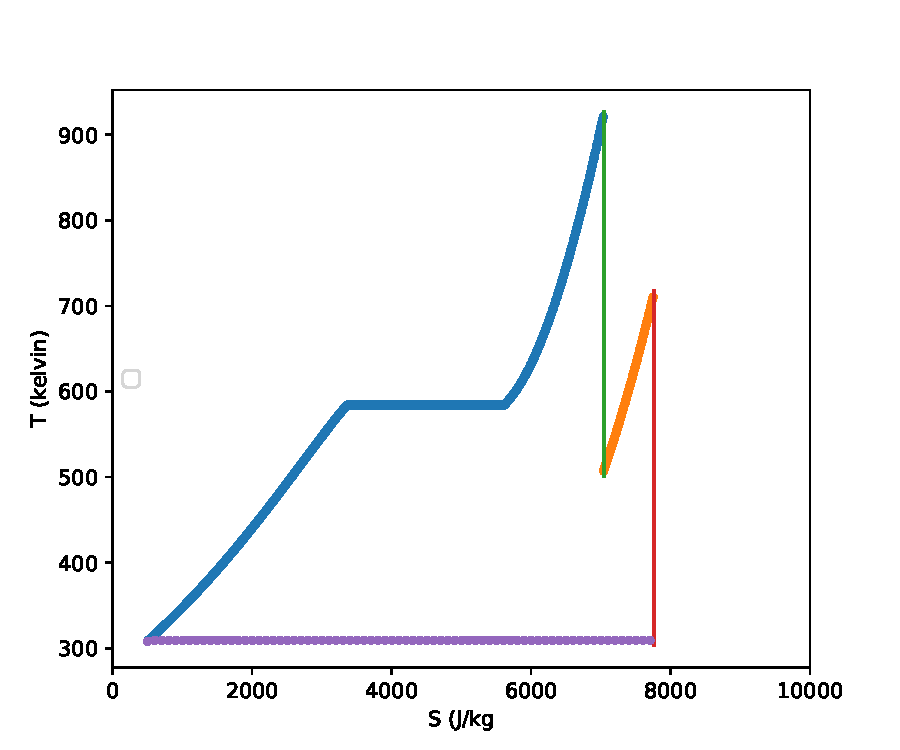
\includegraphics{RankineInitial.pdf}
    \caption{Caption}
    
    \label{fig:my_label}
\end{figure}

\FloatBarrier

\section{Modeling Heat Exchanger}
In order to model the Heat Exchanger a measured effectiveness of 0.85 is used. This is an experimental value for potential heat exchangers on the market.
    \[Effectiveness = 0.85\]
First the mass flow rate of the Brayton cycle is found using the given inputed heat and the mass specific change in enthalpy between state 2 and 3 of the Brayton cycle.
    \[\dot{m} = h_3 - h_2 / \dot{Q}\]
The effectiveness is defined as the actual heat transferred divided by the potential heat transferred.
   \[Effectiveness = actual Q transfer/ Ideal Q transfer\]
The actual heat transfered is defined as the heat input in the rankine cycle, which is the mass flow rate multiplied by the mass specific change in enthalpy between state 3 and 2 of the Rankine cycle.
   \[Qactual = \dot{m} * (h_3 - h_2)\]
The ideal heat transfered is defined as the mass flow rate multiplied by the mass specific change in enthalpy between state 4 and 1 of the Brayton cycle.
    \[Qideal = \dot{m} * (h_4 - h_1)\]
The Mass Flow Rate of the Rankine Cycle can then be found as:
    \[\dot{m}rankine = effectiveness * \dot{m}brayton * (h_4 - h_1)brayton / (h_3 - h_2)rankine\]
Using the MassFlowRate of both cycles the combined Cycle Efficiency can by found by combining the net work per second and Q-in of the cycles.
    \[CombinedEfficiency = netWork/Qin\]
    \[WorkPerSecond = \dot{m} * massSpecificWork\]
    \[QinPerSecond = Qin + \dot{m} * Qin-rankineReheat - \dot{m} * Qout-braytonIntercool\]
    \[netWork = W(rankine) + W(Brayton)\]
After Inputting the initial values used in both cycles, and using these equations a combined Cycle efficiency of 41.50 \% is found. This isn't great, especially considering it is only a slightly larger efficiency than the Brayton cycle, and is a lower efficiency than the Rankine cycle. So it is imperative to improve the efficiency.

\section{Maximising Pressure Ratio Efficiency}
Using the combined cycle model, a different variable for the pressure ratio of the Brayton Cycle is iterated over. A pressure ratio of 1 (no change in pressure) to 40 (already exceeding possible material science) is iterated over. The following graph displays the values for combined cycle efficiency are found.

\begin{figure}
    \centering
    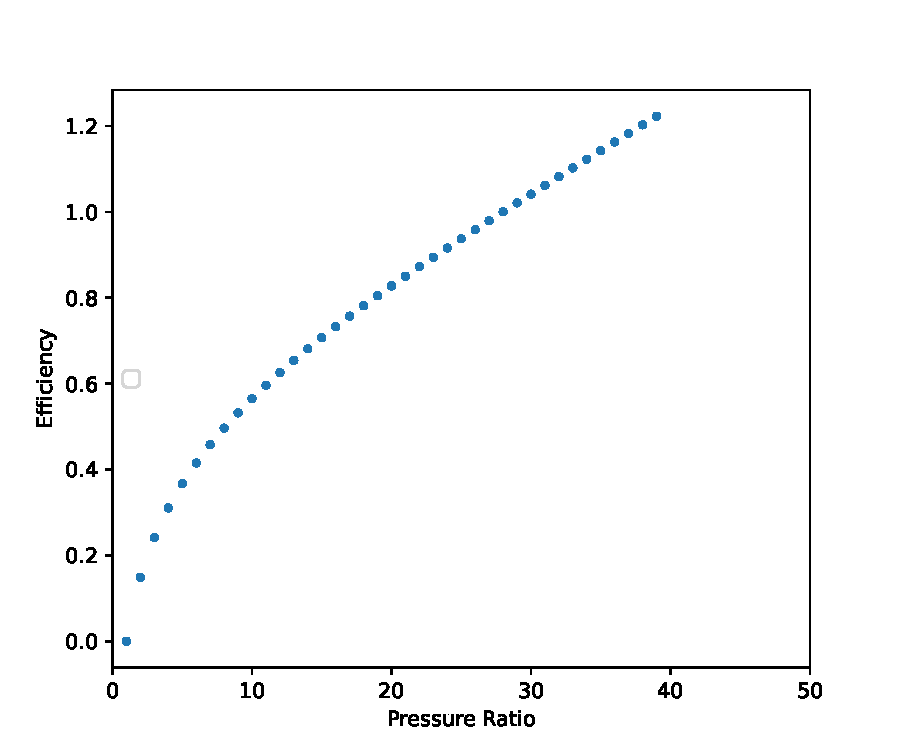
\includegraphics{presureratioefficiencygraph.pdf}
    \caption{}
    
    \label{fig:my_label}
\end{figure}

\FloatBarrier

While efficiency does continue to improve as the pressure ratio increases, it begins to level out in a manner similar to the square root function. So the increase in cost of the actual power plant meets diminishing returns. In order to choose an ideal pressure ratio various power plant component prices would be compared to the theoretical efficiency gains of their operation.

\section{Maximising Efficiency of the Steam Turbine Rankine Cycle}
The first variable that was iterated over was the low pressure of the Rankine cycle (the condenser pressure). The following efficiency graph was produced:

\begin{figure}
    \centering
    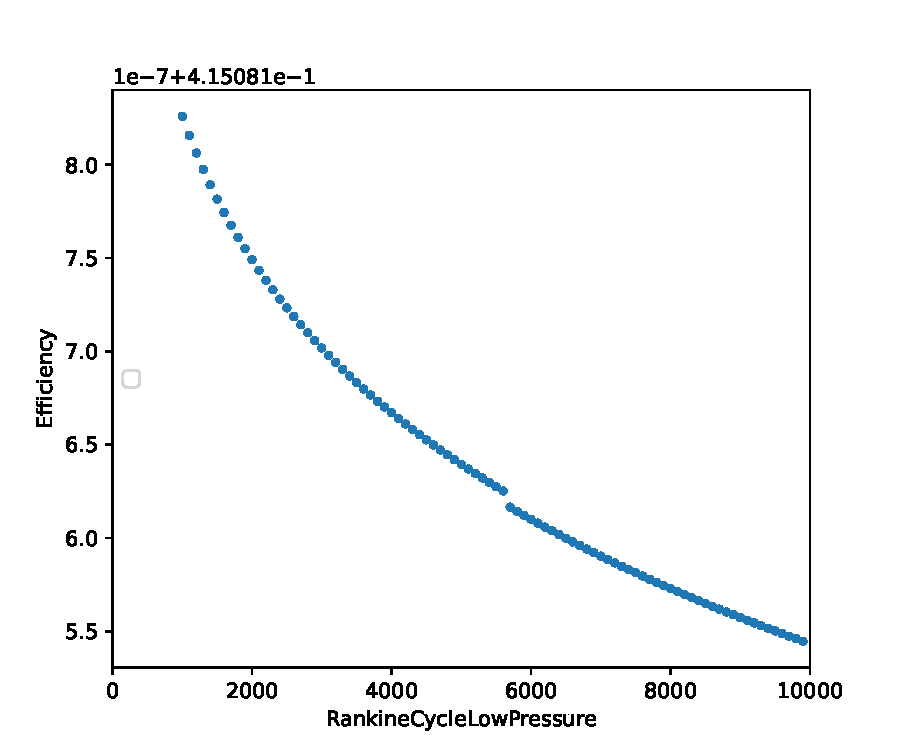
\includegraphics{RankineLowPressureGraph.pdf}
    \caption{Note the scale of the graph; the efficiency does not go over 1}
    
    \label{fig:my_label}
\end{figure}

\FloatBarrier

The lowest pressure possible had the highest efficiency. However, despite the large changes in pressure the combined cycle efficiency changes only in the 4th decimal. So in order to maximise the cost benefit ratio of the power plant the cheapest or most reliable components should be used for the low pressure.
Iterating over the maximum pressure of the steam turbine was next. The following graph displays the results:

\begin{figure}
    \centering
    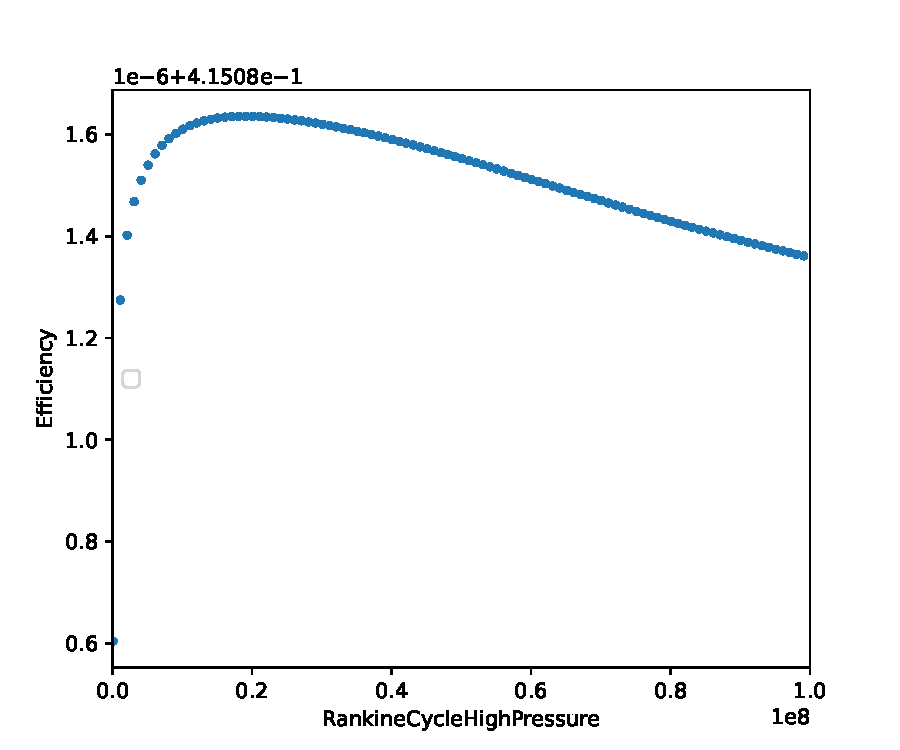
\includegraphics{RankineHighPressureGraph.pdf}
    \caption{Note the scale of the graph; the efficiency does not go over 1}
    
    \label{fig:my_label}
\end{figure}

\FloatBarrier

The graph has a maximum efficiency at 19100000 pascals. However, it is interesting how the graph increases at a rapid rate, then starts to decrease. This is because of the work required to compress the liquid water begins to exceed the gains in generated work.

\section{Results}

Running the combined cycle simulation again, but with the maximum efficient values found (pressure ratio = 39, low pressure = 1000 pa, and high pressure of 19100000) yields a combined cycle efficiency of 74.19 \%. A Brayton cycle pressure ratio of 39, may not be possible with current materials, but it gives a huge combined cycle efficiency. The low pressure of the Rankine cycle adds almost nothing to the efficiency, and the high pressure of the Rankine cycle only adds a couple percent, so the largest increase of efficiency is made by increasing the pressure ratio.

\section{Conclusions}

The combined Rankine and Brayton cycle provide a large thermal efficiency as compared to each individual cycle. The Rankine with reheat only had a thermal efficiency of 46.93 \% and the Brayton with an inter-cooler had a thermal efficiency of 35.67 \%. Once combined and optimised the thermal efficiency reached 74.19 \% (granted I did throttle the pressure ratio beyond current technology). In order to continue to improve the thermal efficiency more modifications could be added to the cycles, and iterating over their state values could yield a much larger efficiency. I did not iterate over all three variables at the same time to save coding and computing time. In order to continue this study to find maximum thermal efficiency of the combined cycle more modifications could be added to the Rankine and Brayton cycle. The Brayton cycle could have a regenerator. And the Rankine Cycle could utilise superheating during the compression stage. Then all the state variables could be iterated over at the same time.

\appendix

\FloatBarrier % To keep all figures before the references

% produces the bibliography section when processed by BibTeX
\bibliography{Paper_template_bib_file}
\bibliographystyle{aiaa}

this = https://github.com/cowblocks/Submission-1

\section*{Code Listing}

\lstinputlisting[language=Python]{Great_Code.py}






\end{document}
